%!TEX root = comps_NKasimov.tex
\chapter{High Fidelity Simulation Results}
\label{chapter:4}
In this chapter one can find  the results of benchmarking for CBVP applied to simple testing problem --- Heat equation with different boundary conditions at the wall (Dirichlet, Neumann, Robin), as well as results of High Fidelity simulations with the use of CBVP for flows around different number and types of obstacles.

\section{Benchmark of using Characteristic Based Volume Penalization}
Applicability of CBVP on different BC is tested on 1D heat equation \eqref{eq:heat}. 
\begin{align}
\frac {\pt T}{\pt t} &= k \frac {\pt^2 T}{\pt x^2}. \label{eq:heat}
\end{align}
On the right domain boundary the wall is placed, so one can observe reflection of the incident wave using CBVP and compare it to exact solution. The main error controlling parameter in CBVP is penalization parameter $\eta$, so it is varied to achieve convergence with exact solution.

\subsection{Dirichlet Boundary Condition}
This boundary condition \eqref{eq:heat_dirichlet}, also called isothermal boundary condition, specifies temperature (integrated variable for heat equation) as a constant value at the obstacle/wall interface. In this particular benchmark the value is equal to 0.
\begin{align}
\vbr T_{wall} = 0 \qquad \implies \qquad \frac {\pt T}{\pt t} &= k \frac {\pt^2 T}{\pt x^2} - \frac \chi \eta_b T. \label{eq:heat_dirichlet}
\end{align}
Varying penalization parameter $\eta_b$ led to solutions with different accuracy (see Fig.~\ref{fig:heat_dirichlet}).
\begin{figure}[h!]
\centering 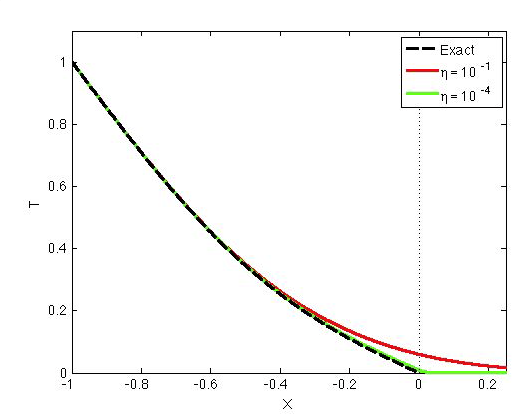
\includegraphics[scale=0.6]{fig/heat_dirichlet.png}\\
\caption{Temperature profile at the end of simulation. Dirichlet boundary condition \label{fig:heat_dirichlet}}
\end{figure}\\
One can see that $\eta_b = 10^{-4}$ converges to the exact solution well. In fact, rate of convergence for this simulation is $\sqrt{\eta_b}$ \cite{ebd_nk_ovv_cbvp_jcp}, since it is Brinkman type penalization \cite{lib:vp_liu}.

\subsection{Neumann Boundary Condition}
This boundary condition \eqref{eq:heat_neumann} specifies constant rate of heat amount going in to or out of the system. In case of zero rate it is called adiabatic boundary condition. In this benchmark latter is considered.
\begin{align}
\vbr{\frac {\pt T}{\pt x}}_{wall} = 0 \qquad \implies \qquad \frac {\pt T}{\pt t} &= (1-\chi)k \frac {\pt^2 T}{\pt x^2} - \frac \chi \eta_c \frac {\pt T}{\pt x}. \label{eq:heat_neumann}
\end{align}
Analogously to Dirichlet BC, varying penalization parameter $\eta_c$ led to different accuracy of the solution (see Fig.~\ref{fig:heat_neumann}). Rate of convergence for this type of simulations is $\eta_c$ \cite{ebd_nk_ovv_cbvp_jcp}. One can notice that penalization parameter for Neumann type BC is different than for Dirichlet type BC, which is connected to different time scales of the processes. In case of BP solution at the boundary decays inside of the obstacle, on the other hand for characteristic BC solution is translated inside of the obstacle. 
\begin{figure}[h!]
\centering 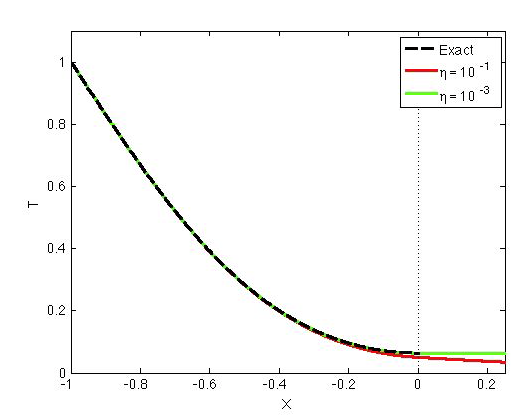
\includegraphics[scale=0.6]{fig/heat_neumann.png}\\
\caption{Temperature profile at the end of simulation. Neumann boundary condition \label{fig:heat_neumann}}
\end{figure}

\subsection{Robin Boundary Condition}
Last benchmark problem is to mimic Robin boundary condition at the obstacle interface, when both the solution value and its derivative are specified at the boundary. In this particular problem \eqref{eq:heat_robin} is used as a BC.
\begin{align}
T + 2 \frac {\pt T}{\pt x} = 5 \qquad \implies \qquad \frac {\pt T}{\pt t} &= (1-\chi)k \frac {\pt^2 T}{\pt x^2} - \frac \chi {\eta_r} \rbr{T + 2 \frac {\pt T}{\pt x} - 5}. \label{eq:heat_robin}
\end{align}
In this type of simulations rate of convergence is predominated due to characteristic based terms as $\eta_r$ \cite{ebd_nk_ovv_cbvp_jcp} (see Fig.~\ref{fig:heat_robin}).
\begin{figure}[h!]
\centering 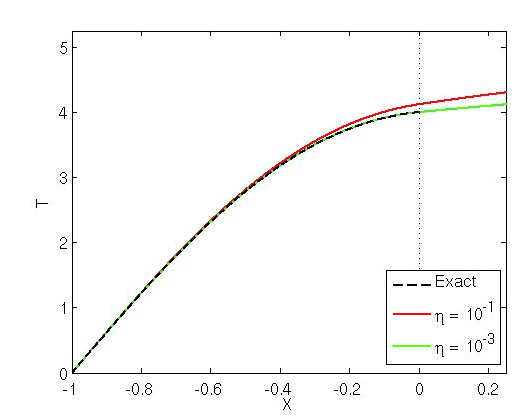
\includegraphics[scale=0.6]{fig/heat_robin.png}\\
\caption{Temperature profile at the end of simulation. Robin boundary condition \label{fig:heat_robin}}
\end{figure} 

\section{Simulation Results}
After the method is validated and convergence rates are studied, variety of 2D simulations of supersonic inviscid flow are performed. Namely, flow around single and multiple stationary and moving cylinders, wedges with subcritical and supercritical angles. It is worth to mention that at this point no quantitative analysis of applicability of CBVP is done for these simulations. All results are treated based on the assumption that convergence rates defined in heat equation benchmarks hold for these simulations according to the used BCs (either $\sim \sqrt \eta$ or $\sim \eta$). 

\subsection{Flow around the Wedge}
In this set of simulations supersonic flow around both subcritical and supercritical wedges are considered. Incident shock speed is $M = 1.5$ (see Fig.~\ref{fig:wedge_scheme}). In case of subcritical wedge, i.e. angle at the apex is less than certain critical angle $\theta_{crit}$, secondary oblique shock is formed. 
\begin{figure}[h!]
\centering 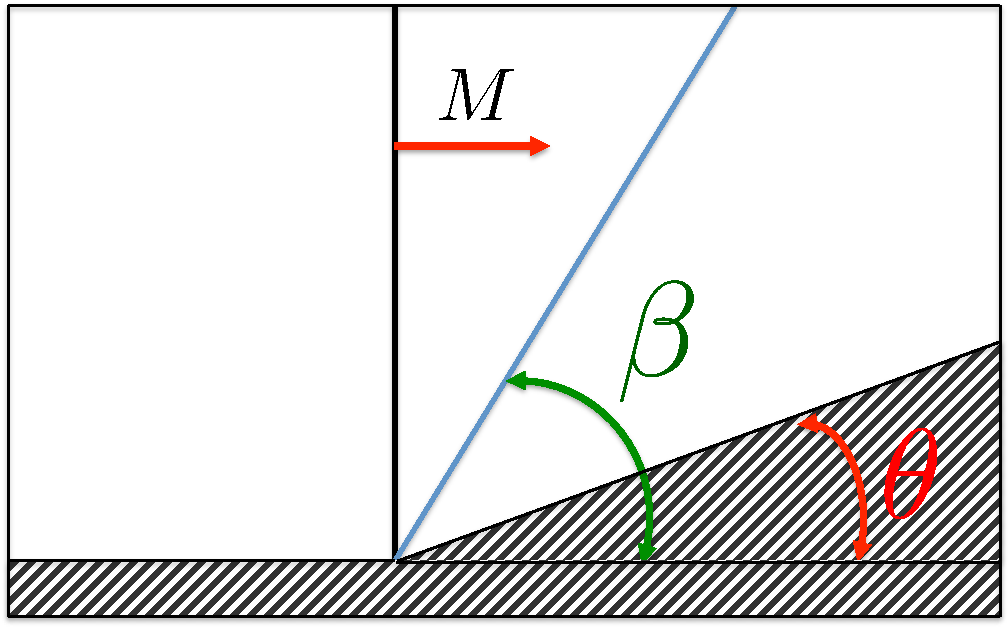
\includegraphics[scale=0.6]{fig/wedge_scheme.pdf}\\
\caption{Schematic of the flow around the wedge \label{fig:wedge_scheme}}
\end{figure}\\
Between the wedge angle $\theta$ and oblique shock deflection angle $\beta$ there is a relation called ``$\theta-\beta-M$'' equation \eqref{eq:th-b-m} (see Fig.~\ref{fig:th-b-m}).
\begin{align}
\tan \theta = 2 \cot \gb \frac {M \sin^2 \gb - 1}{M^2 \rbr{\gG + \cos 2 \gb} + 2}. \label{eq:th-b-m}
\end{align}
\begin{figure}[h!]
\centering 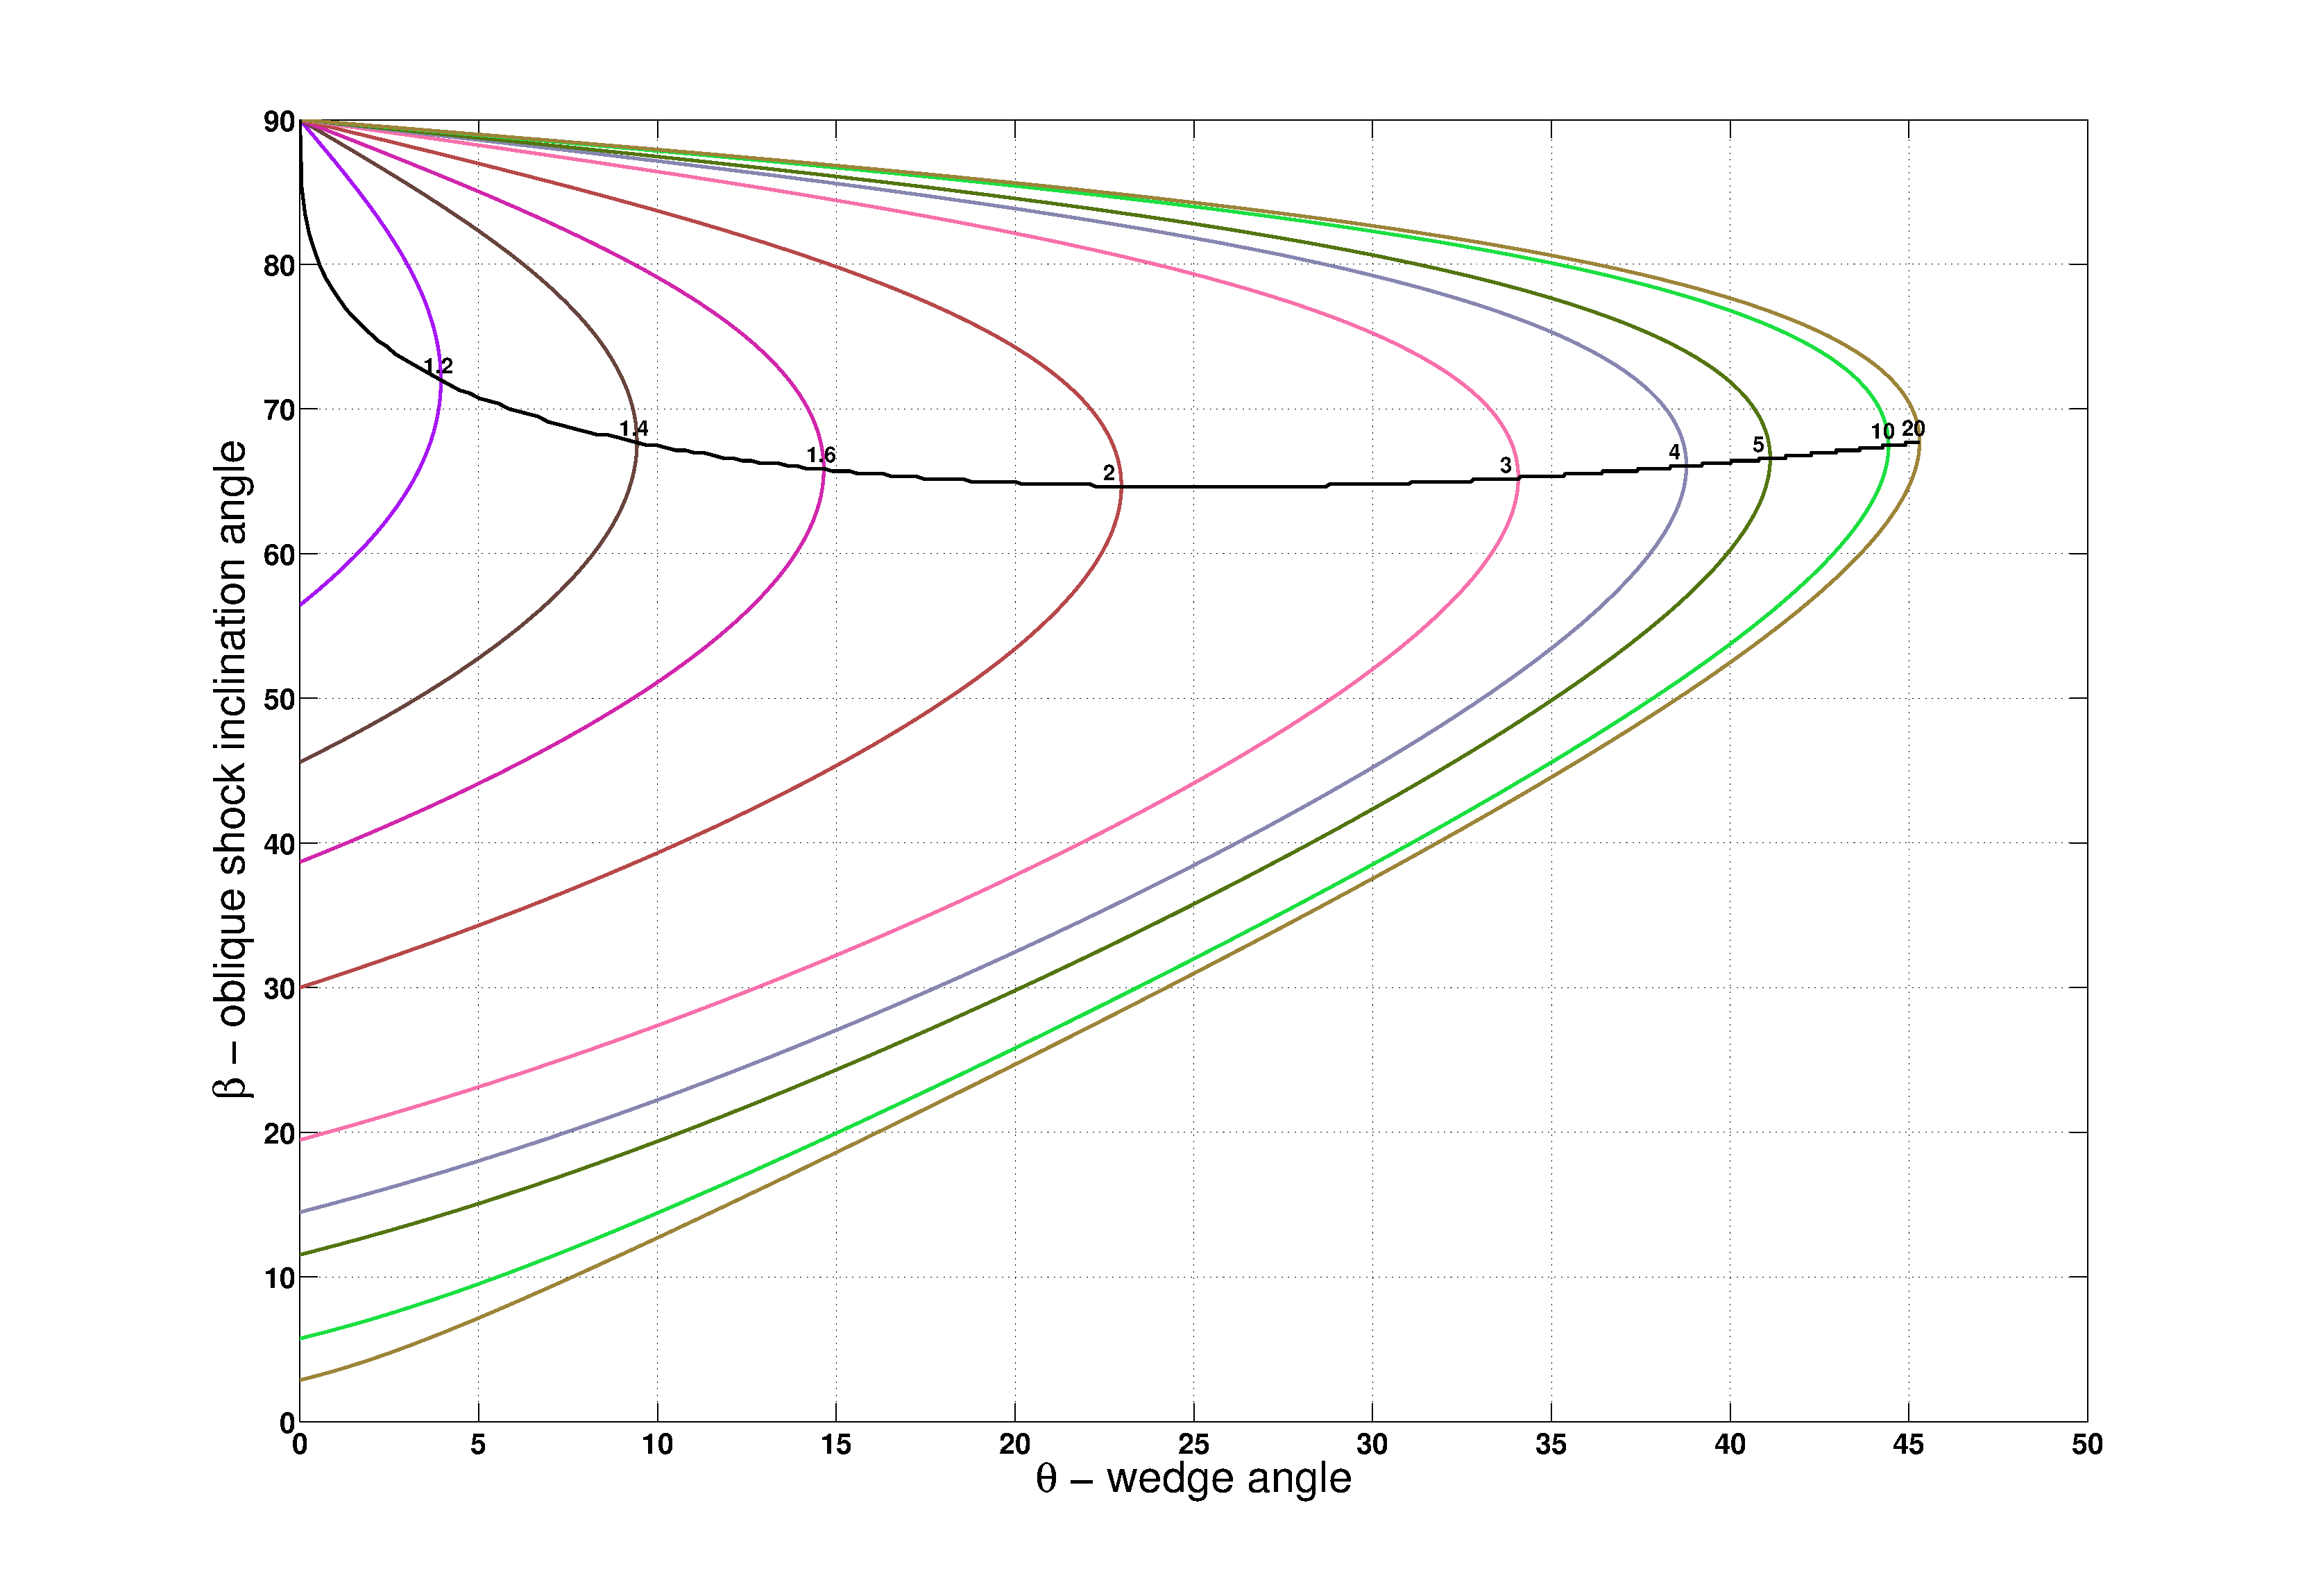
\includegraphics[scale=0.2]{fig/th-b-m.pdf}\\
\caption{$\theta-\beta-M$ relation plot \label{fig:th-b-m}}
\end{figure}\\
For this particular setup, one can find that $\theta_{crit} \approx 15^\circ$, and subcritical wedge angle is $\theta = 10^\circ$. For the wedge angle $\theta > \theta_{crit}$ detached bow shock is formed. Supercritical angle is $\theta = 25^\circ$.
\begin{figure}[h!]
\centering 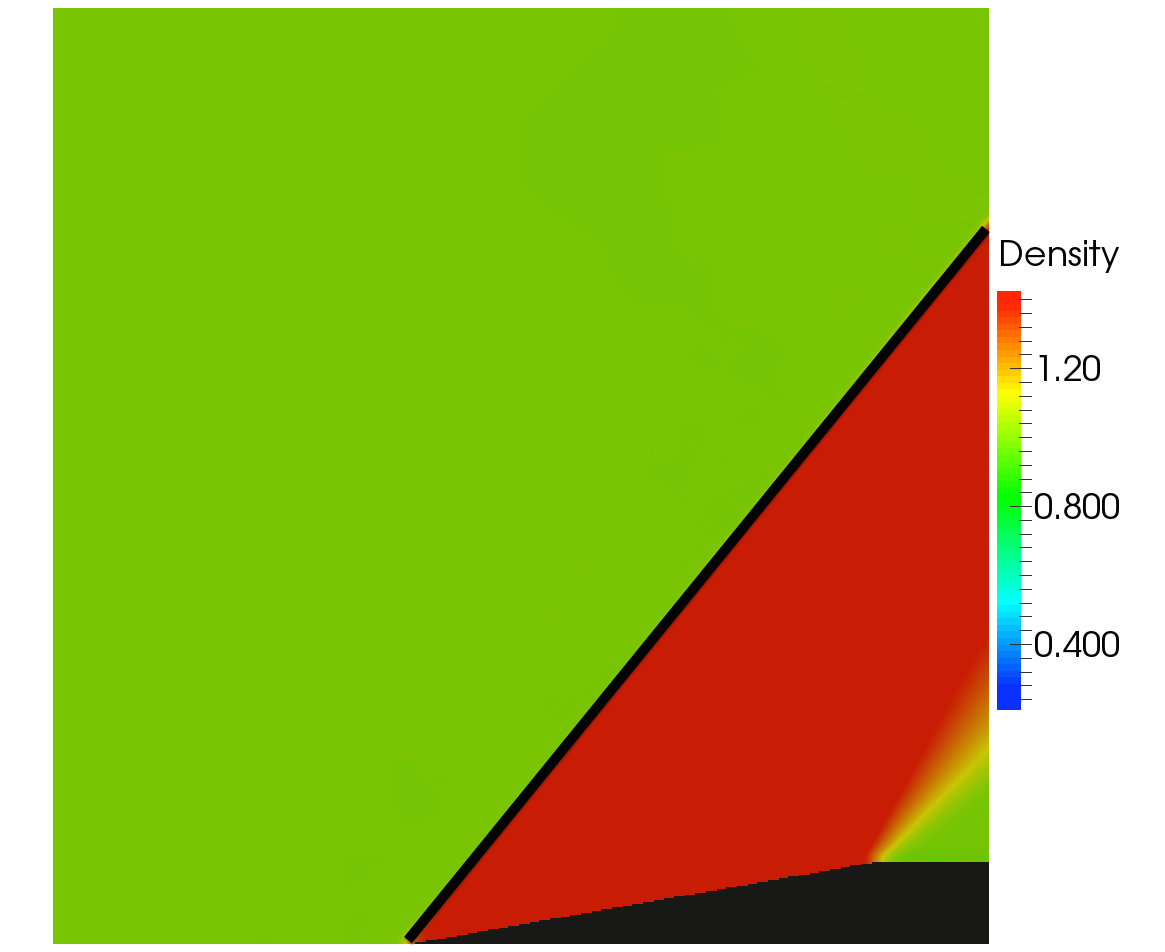
\includegraphics[width=0.69\linewidth]{fig/wedge_sub.png}\\
Subcritical wedge\\ [1ex]
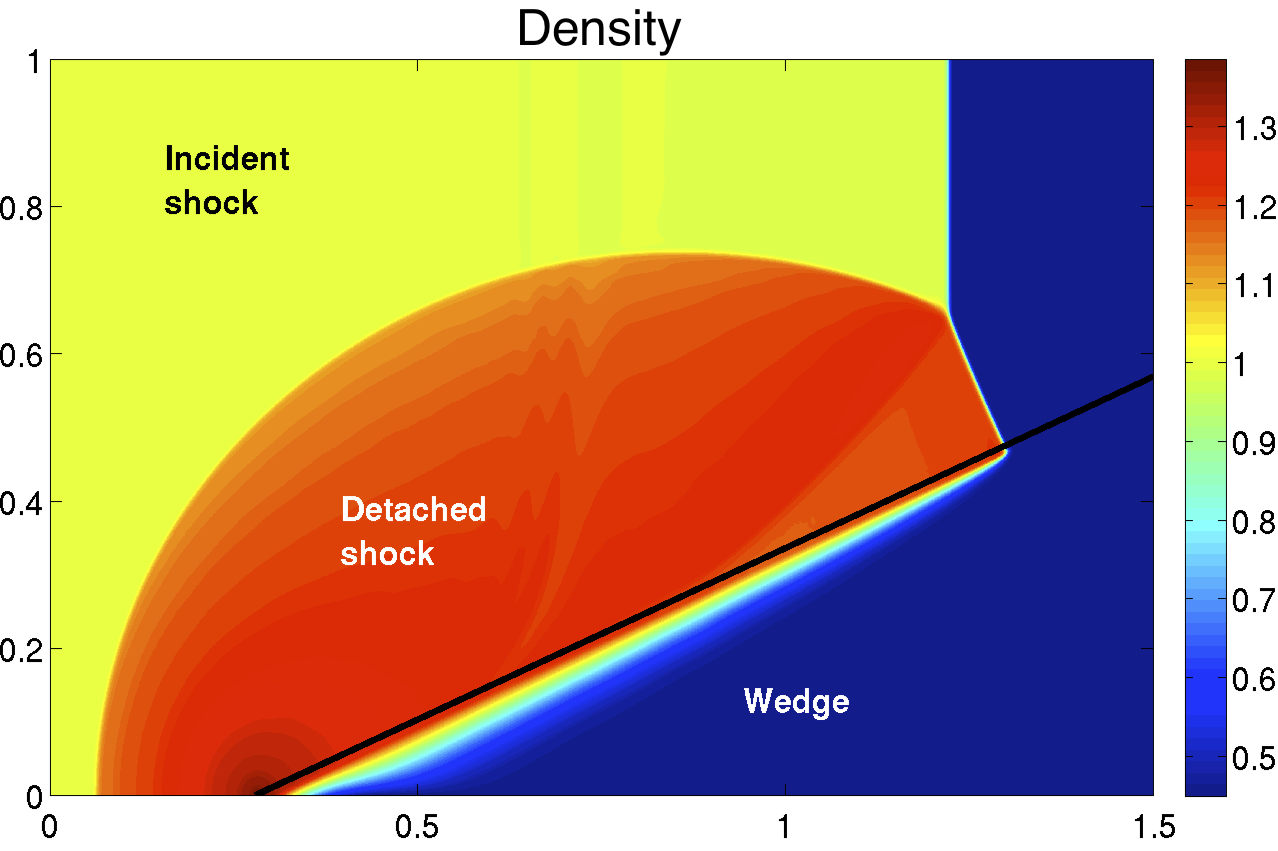
\includegraphics[width=0.65\linewidth]{fig/wedge_super.png}\\
Supercritical wedge\\
\caption{Flow around the wedge results \label{fig:wedge_res}}
\end{figure}

\subsection{Flow around Single and Multiple Stationary Cylinders}
In this set of simulations, same $M=1.5$ shock impinges either single or multiple solid cylinders (see Fig.~\ref{fig:cyl_scheme}). Unlike the flow around the wedge, in case of cylinder always detached shock will be formed. There is no analytical solution to this problem.
\begin{figure}[t]
\begin{minipage}{0.5\linewidth}
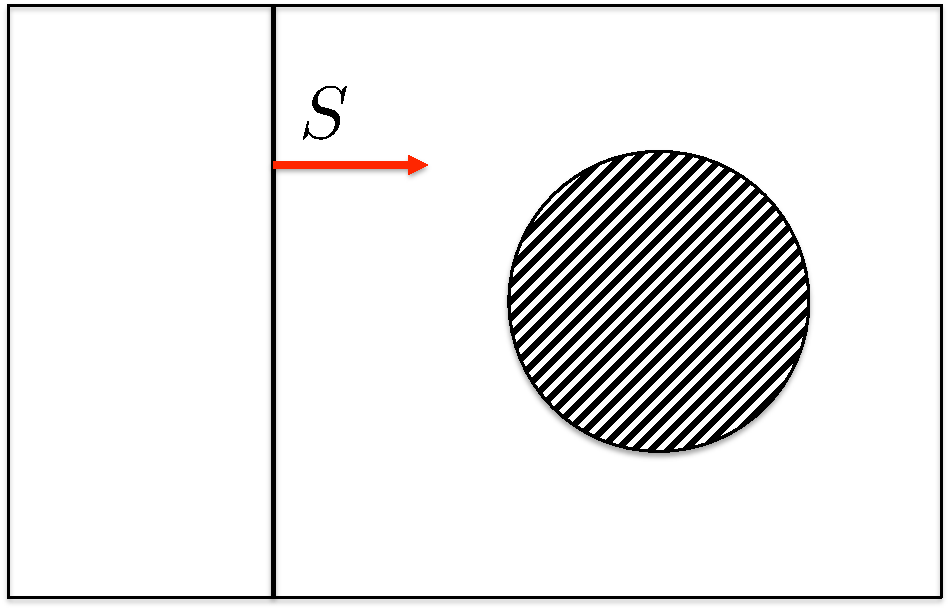
\includegraphics[scale=0.4]{fig/single_cyl.pdf}
\end{minipage}
\begin{minipage}{0.5\linewidth}
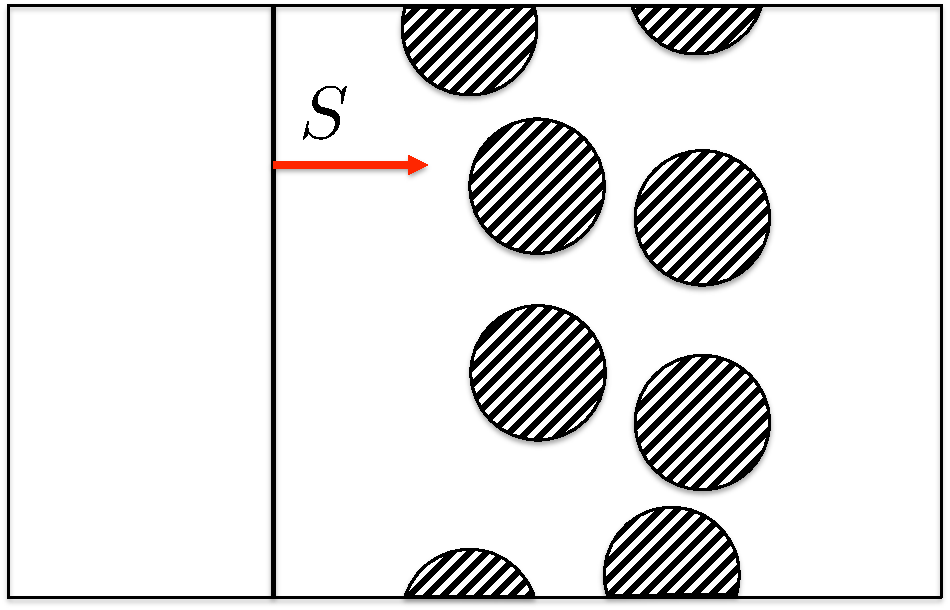
\includegraphics[scale=0.4]{fig/mul_cyl.pdf}
\end{minipage}
\caption{Single and multiple cylinders case schematics} \label{fig:cyl_scheme}
\end{figure}\\
In case of single cylinder, one can see reflected bow shape shock (see Fig.~\ref{fig:single_res}).
\begin{figure}[h!]
\centering 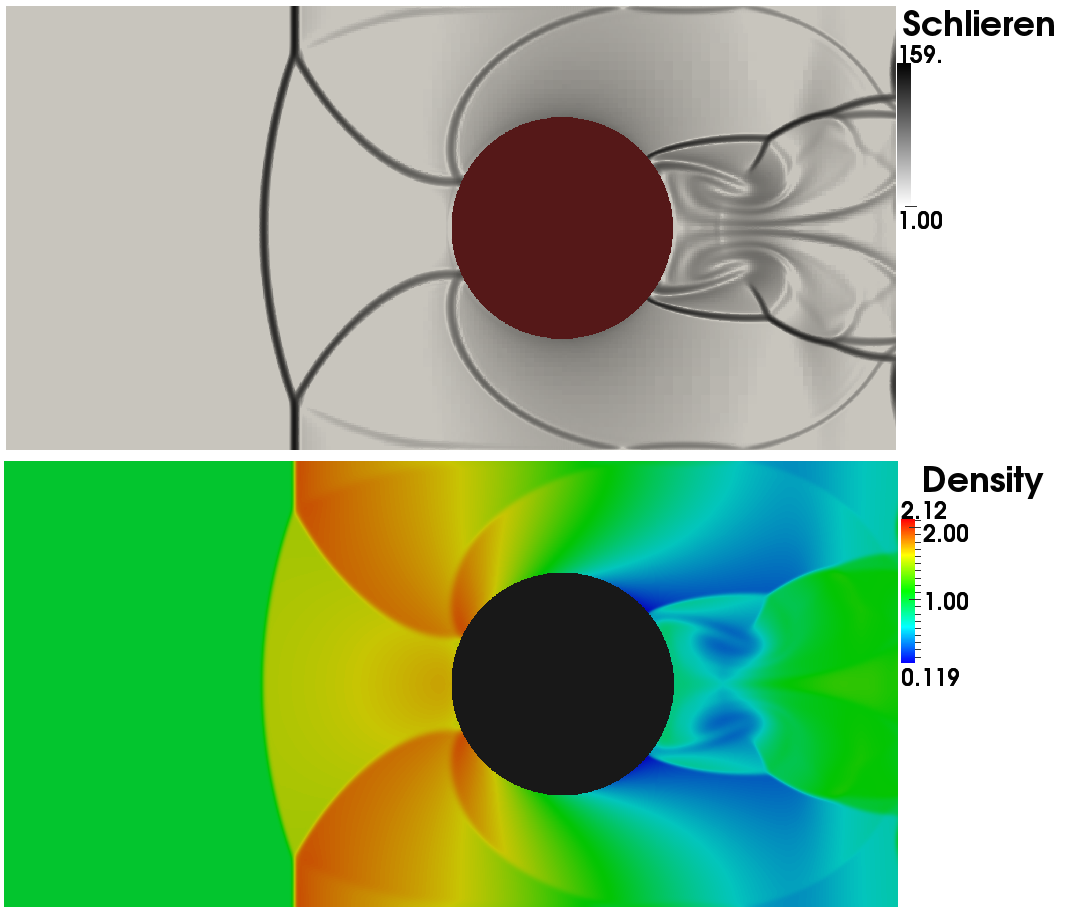
\includegraphics[scale=0.3]{fig/single_res.png}\\
\caption{Supersonic flow around single cylinder \label{fig:single_res}}
\end{figure} \\
In case of multiple cylinders one can also notice shock-shock interactions (see Fig.~\ref{fig:mult_res}). \\\\\\
\begin{figure}[t]
\centering 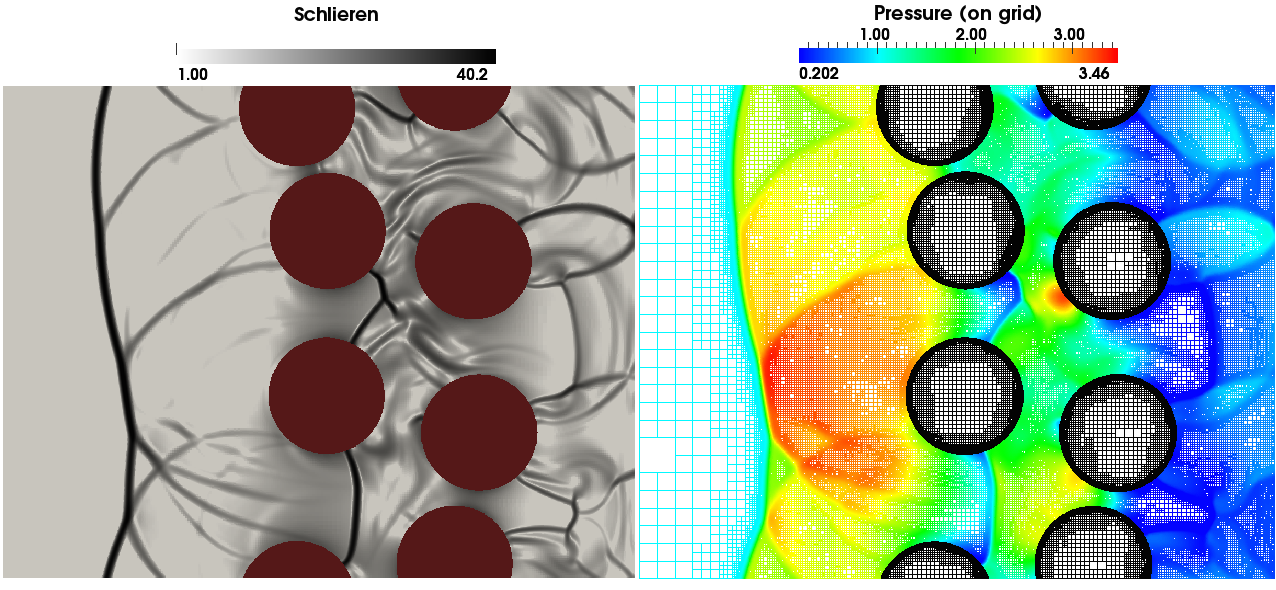
\includegraphics[scale=0.35]{fig/mult_res.png}\\
\caption{Supersonic flow around multiple cylinders \label{fig:mult_res}}
\end{figure}
\begin{figure}[h!]
\centering 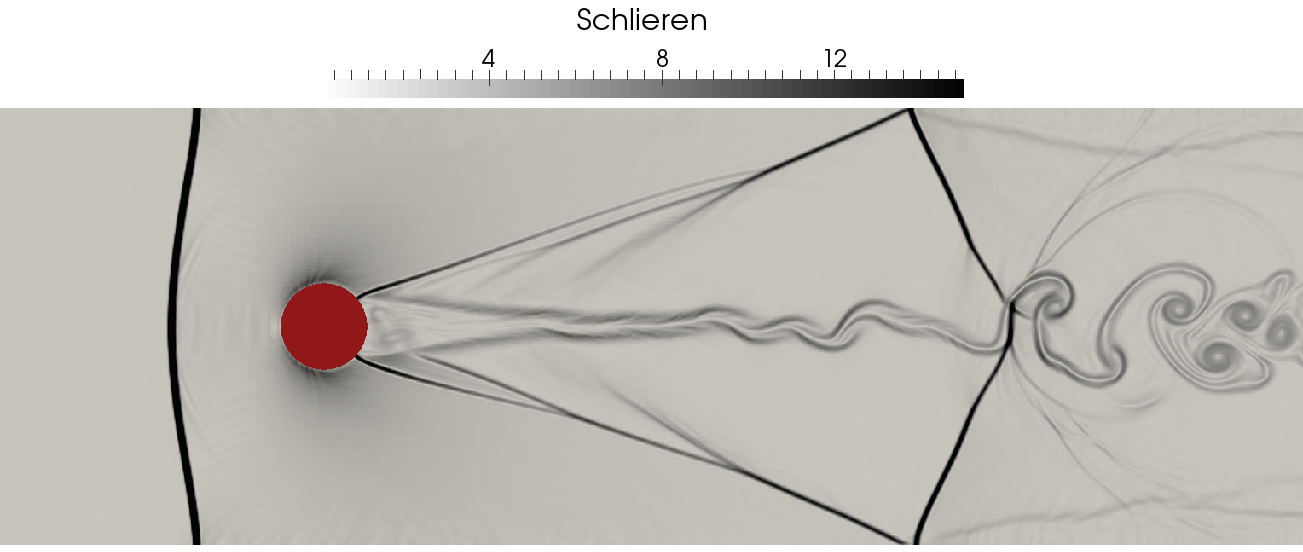
\includegraphics[scale=0.21]{fig/nonmov_res.png}\\
\centering 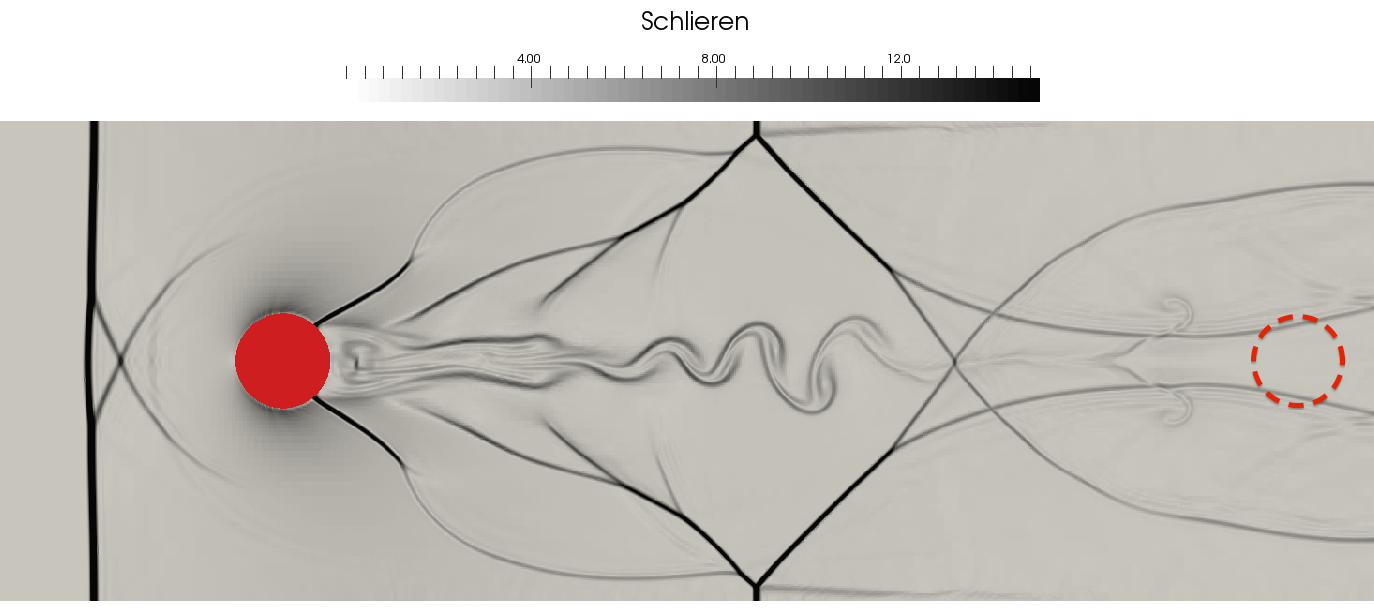
\includegraphics[scale=0.2]{fig/moving_res.png}
\caption{Supersonic flow around stationary and moving cylinders \label{fig:mov_res}}
\end{figure}
\subsection{Flow around Single Stationary and Moving Cylinder}
This case is to demonstrate the ability of the CBVP to handle physically equivalent phenomena considered from two different frame of references, moving and non moving, within the acceptable level accuracy. For this purpose, two identical numerical frameworks are developed. One with supersonic uniform background flow and stationary cylinder, and another with zero background flow and a single cylinder moving supersonically embedded to that flow. Flow pressure and density are kept identical in both set ups (see Fig.~\ref{fig:mov_res}). One can notice that results are not completely identical. The reason is at this point methodology is not completely consistent when switching to moving frame of reference, and this issue will be addressed in future work (see Chapter~6).